\section{Работа с коллекциями}
\subsection{Условие задания}
Выполнить задание. Вариант: <<Создать двусвязный список, состоящий из целых чисел. Найти сумму элементов, попадающих в заданный интервал [a, b]. Получить новый список, вставив после каждого четного элемента новый элемент>>.

Разработать приложение в соответствии со своим вариантом.

Приложение должно выполнять следующие действия:

\begin{enumerate}
\item Заголовок формы должен отражать суть задания.
\item Все элементы формы должны быть внятно подписаны (кнопки подписаны, у тестового поля должно быть написано, для чего оно нужно и т. д.)
\item В коде должны быть комментарии и отступы (код должен быть легко читаем).
\item В коде программы все элементы формы должны быть переименованы (btnName -  для кнопок, lblName - для ссылок, txtName - для текстового поля и т.д.) Наименования должны быть понятными.
\item Должна быть возможность для ввода и вывода первоначальных данных.
\item Должна быть возможность для вставки и удаления одного элемента.
\item Должны использоваться коллекции.
\item Ответы на задания должны быть в разных полях.
\item Если нет данных для выполнения задания, выводить соответствующие данные.
\item Для графов использовать список смежности.
\end{enumerate}

\subsection{Вид формы в конструкторе}
Форма имеет вид как на рисунке \ref{fig:collections-form}

\begin{figure}
\centering
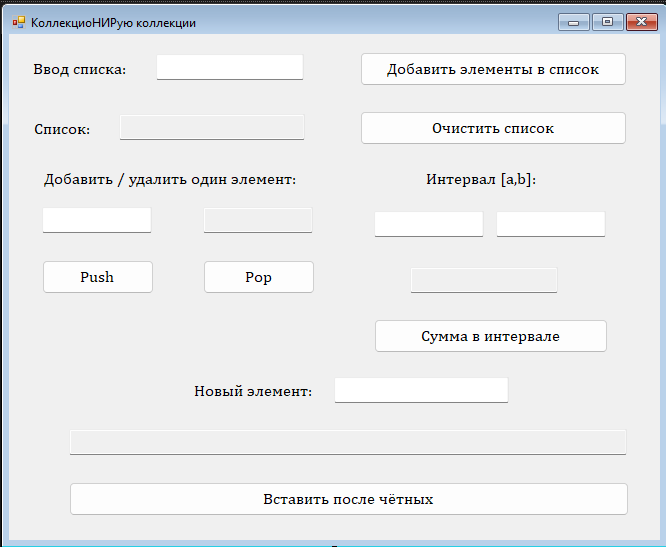
\includegraphics[width=0.5\linewidth]{images/collections/form.png}
\caption{Форма окна для задания}
\label{fig:collections-form}
\end{figure}

\subsection{Таблица с описанием элементов формы}
Все элементы формы были переименованы для большей читаемости. В таблице \ref{tab:collections-form} представлены все изменения.


\begin{xltabular}{\textwidth}{| m{0.3\textwidth} | m{0.3\textwidth} | m{0.3\textwidth} |}

\hline
\textbf{Описание элементов формы} & \textbf{Список изменённых атрибутов} & \textbf{Новое значение атрибута} \\
\hline
\endfirsthead

\hline
\textbf{Описание элементов формы} & \textbf{Список изменённых атрибутов} & \textbf{Новое значение атрибута} \\
\hline
\endhead

\hline
\endfoot

\hline
\caption{Значение атрибутов элементов в приложении для работы с коллекциями}
\label{tab:collections-form}
\endlastfoot

Окно формы & Text & КоллекциоНИРую коллекции \\
Метка <<Ввод списка>> & Name & lbl1 \\
Метка <<Список>> & Name & lbl2 \\
Метка <<Добавить/удалить один элемент>> & Name & lbl3 \\
Метка <<Интервал [a,b]>> & Name & lbl4 \\
Метка <<Новый элемент>> & Name & lbl5 \\

Поле ввода для списка & Name & listInput \\
Поле вывода для списка & Name & listOutput \\

Поле ввода для добавления элемента & Name & elPush \\
Поле вывода для удалённого элемента & Name & elPop \\

Поле ввода для левой границы интервала & Name & leftInt \\
Поле ввода для правой границы интервала & Name & rightInt \\

Поле вывода для суммы в интервале & Name & sumInt \\

Поле ввода для нового элемента, вставленного определённым образом & Name & newEl \\
Поле вывода для обновлённого списка & Name & listNewOutput \\

Кнопка <<Добавить элементы в список>> & Name & btnInputList \\
Кнопка <<Очистить список>> & Name & btnClearList \\
Кнопка <<Сумма в интервале>> & Name & btnSum \\
Кнопка <<Вставить после чётных>> & Name & btnNewAfterMax \\
Кнопка <<Push>> & Name & btnPush \\
Кнопка <<Pop>> & Name & btnPop \\
Проводник ошибок & Name & eP1 \\
\end{xltabular}


\subsection{Примеры правильной и неправильной работы приложения}
При запуске приложения на экране появляется окно \ref{fig:collections-start}.

\begin{figure}
\centering
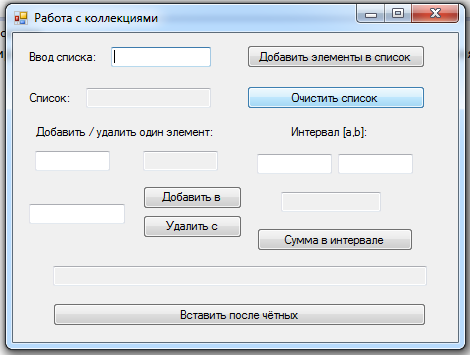
\includegraphics[width=0.5\linewidth]{images//collections/start.png}
\caption{Запуск программы}
\label{fig:collections-start}
\end{figure}

При нажатии на кнопку всё обрабатывается корректно. Также происходит обработка ошибок.

\begin{figure}
\centering
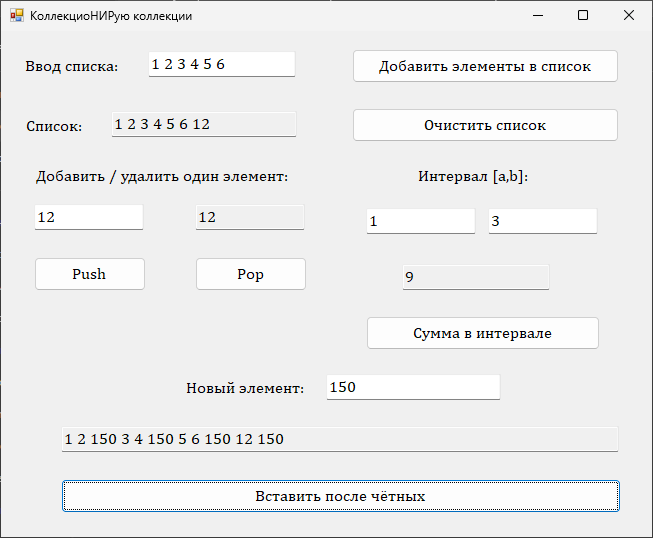
\includegraphics[width=0.5\linewidth]{images//collections/okay.png}
\caption{Запуск с корректными данными}
\label{fig:collections-okay}
\end{figure}

\begin{figure}
\centering
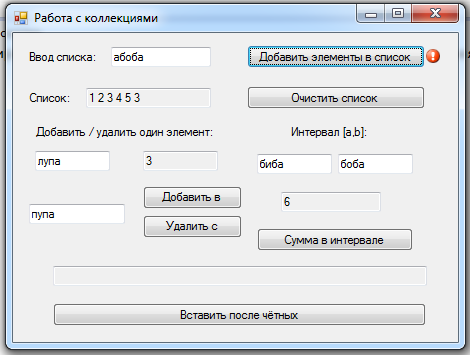
\includegraphics[width=0.5\linewidth]{images//collections/error.png}
\caption{Пример ввода с некорректными данными}
\label{fig:collections-error}
\end{figure}

\begin{figure}
\centering
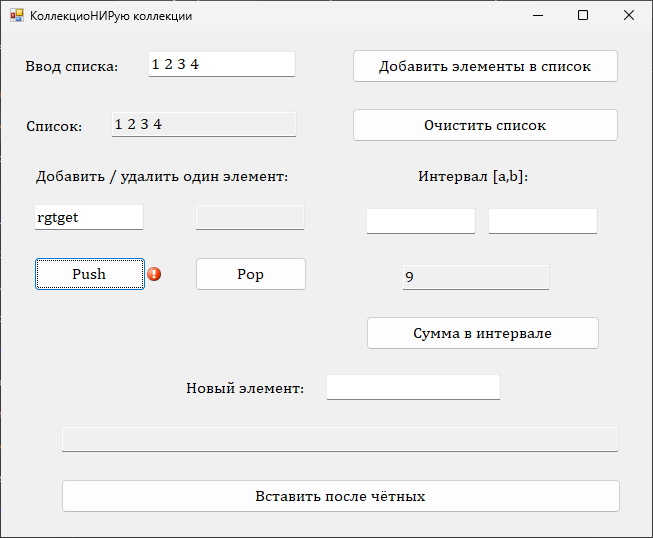
\includegraphics[width=0.5\linewidth]{images//collections/error2.png}
\caption{Пример ввода с некорректными данными}
\label{fig:collections-error2}
\end{figure}

\begin{figure}
\centering
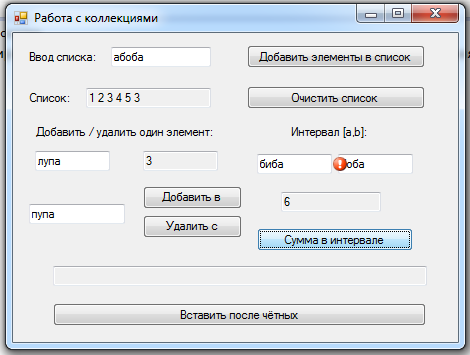
\includegraphics[width=0.5\linewidth]{images//collections/error3.png}
\caption{Пример ввода с некорректными данными}
\label{fig:collections-error2}
\end{figure}

\subsection{Примеры исходного кода}
\begin{minted}{cpp}
/* функция для вычисления суммы в интервале списка */
private: System::Void btnSum_Click(System::Object^ sender, System::EventArgs^ e) {
    ClearAll();
    
    int a, b;
    bool resA = Int32::TryParse(leftInt->Text, a);
    bool resB = Int32::TryParse(rightInt->Text, b);
    int sum = 0, i = 0;
    
    if (!resA) {
        this->eP1->SetError(leftInt, "Не целое число");
        return;
    }
    if (!resB) {
        this->eP1->SetError(rightInt, "Не целое число");
        return;
    }
    if (a < 0 || a > b || a > listState.Count) {
        this->eP1->SetError(leftInt, "Неверный интервал");
        return;
    }
    if (b > listState.Count) {
        this->eP1->SetError(rightInt, "Неверный интервал");
        return;
    }

    for each (int^ item in listState) {
        if (item >= a && item <= b) {
            sum += listState[item];
        }
    }

    this->sumInt->Text = Convert::ToString(sum);
}
\end{minted}

Больше кода проекта доступно в приложении \ref{application-A}. Также в приложенном архиве можно найти полный код проекта.